\documentclass[11pt]{article}
\usepackage{amsmath,amsfonts,amssymb}
\usepackage{graphicx}
\usepackage{subfig}
\usepackage[numbers, sort]{natbib}
\usepackage{hyperref}
\setlength{\topmargin}{-0.5in}
\setlength{\evensidemargin}{0in}
\setlength{\oddsidemargin}{0in}
\setlength{\textwidth}{6.5in}
\setlength{\textheight}{9in}
 \setlength{\parindent}{0in}
 
 \long\def\symbolfootnote[#1]#2{\begingroup\def\thefootnote{\fnsymbol{footnote}}
\footnote[#1]{#2}\endgroup}

\newcommand{\be}{\begin{equation}}
\newcommand{\ee}{\end{equation}}
\newcommand{\ba}{\begin{eqnarray}}
\newcommand{\ea}{\end{eqnarray}}


%%%%%%%%%%%%%%%%%%%%%%%%%%%%%%%%%%%%%%%%%%
%%%%%%%%%

\title{E866/NuSea data in NNPDF}
\author{nh}
\begin{document}
\maketitle
Fixed target Drell-Yan data from the E866/NuSea experiment is used in two forms in NNPDF.
Firstly the $pd$ / $pp$ cross-section ratios of~\cite{Towell:2001nh} and secondly the absolute
$pp$ differential cross-section measurements of ~\cite{Webb:2003ps}. Here we shall discuss the
two experiments and their implementation in the NNPDF code.

Data was taken with an 800 GeV proton beam upon hydrogen and deuterium gas targets with collisions
consequently taking place at a hadron-hadron centre of mass energy of $\sqrt{s}=38.8$ GeV.

For each dimuon event, the invariant mass $M$ and the longitudinal momentum $p_{||}$ of the pair
were reconstructed. At leading order one can then make the identification

\be x_F = \frac{p_{||}}{\sqrt{s}/2} = x_1 - x_2, \ee

and

\be M^2 = x_1x_2s. \ee
One can further extract
\be x_2 = XXX\ee
which can be identified with the momentum fraction of the target parton at leading order.
\section{E866R}
Data is presented as cross-section ratios $\sigma_{pd}/2\sigma_{pp}$ in bins of $x_2$.
Data is taken in three spectrometer configurations, sensitive to low, medium and high invariant
masses respectively. In order to remove areas of the spectrum with very poor sensitivity, along with the $J/\psi$ and $\Upsilon$ resonances,
the three different spectrometer configurations use three different sets of invariant mass cuts to define the fiducial region. These are shown
in Table~\ref{tab:massregions}.

\begin{figure}
  \begin{center}
  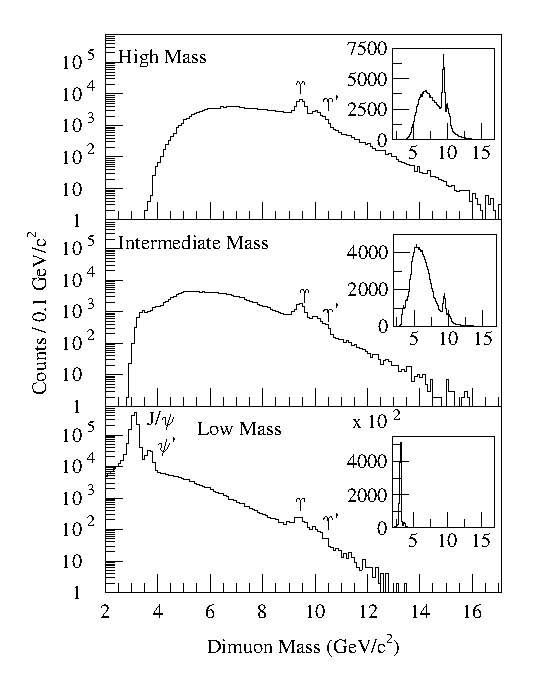
\includegraphics{fig2.eps}}
    \vspace*{-0.05in}                                
  \end{center}       
  \caption{The dimuon mass distributions for the three different mass settings. Taken from \cite{Towell:2001nh}}
  \label{fig:3mass}                    
\end{figure}      


\begin{table}
\begin{center}                                                          
\begin{tabular}{ccc}               
 mass setting	 & mass regions accepted    \\ \hline
 low	      & 4.0 to 8.8 \rm{GeV/c$^2$}   \\ 
 intermediate         & 4.3 to 8.8 \rm{GeV/c$^2$} and $> 10.8$ \rm{GeV/c$^2$}   \\
 high  	      & 4.5 to 9.0 \rm{GeV/c$^2$} and $> 10.7$ \rm{GeV/c$^2$} \\
\end{tabular}
\caption{Mass regions used for each spectrometer settings. Taken from \cite{Towell:2001nh}}
\label{tab:massregions}   
\end{center}
\end{table}

In each mass setting $i$, the E866 collaboration measure (roughly speaking)
\be \sigma^i_{px} = \int dM \frac{d\sigma_{px}}{dM} \Theta^i(M)\epsilon^i(M) \ee
where $\Theta^i(M)$ are the acceptances for mass setting $i$ in Table~\ref{tab:massregions} and
$\epsilon^i(M)$ are the detector efficiencies for mass setting $i$. Crucially in the E866R analysis
these efficiencies are neither provided or really studied at all. No attempt is made to unfold the result for
these detector effects. The final result for $\sigma_{px}$ is then given as a simple average over
the three mass settings.

There are therefore two principle causes for difficulty in making theoretical comparisons to the data, both arising from the presentation of the data inclusive in $M$.
\begin{itemize}
	\item \textbf{Fiducial cross-sections} \\
		The measured cross-sections ratios are not extrapolated to the full mass spectrum.
		This would not generate too much difficulty if we used data from the different spectrometer
		settings separately. But as we use the average, it makes determining the fiducial region complicated.
	\item \textbf{Detector effects} \\
		The mass spectrum is further tainted by detector efficiencies that are not taken into account.
\end{itemize}


While it has been previously assumed that these effects should cancel in the ratio, this is not guarunteed (and indeed is
not an assumption made by the NuSea collaboration). As there is no attempt made in the NuSea paper to quantify the size of these effects, 
there is essentially a missing systematic error on the data whose size is difficult to estimate.

Three methods for making comparison to the data have been attempted.
\subsection{The NuSea method}
The thesis of R.~Towell~\cite{Towell:2001dz} describes the method used by the NuSea collaboration
to make theoretical comparisons to their data. Here they are aware of the limitations of their analysis and do not assume
that the effects of the complicated fiducial region in $M$ or their selection effects cancel in the ratio.

In order to take into account these effects, they perform their computation using the kinematics recorded in their
actual data sample. For each measured event, they compute the corresponding differential cross section according
to its kinematics. The computed differential cross sections are then averaged over the $x_2$ bins used in the analysis.
In this way they can quite accurately take into account the effects of their fiducial region and selection effects. Unfortunately
however as we do not have access to their original event record this is not an option for us.

\subsection{The NNPDF method}
In the current configuration, we approximate that any detector selection effects cancel in the ratio, and
that the average value of the cross-sections over the mass range is well approximated by the cross section at
the average mass value. Specifically we convert the data kinematics from $x_2, M$ to $y, M$ and compute
\be R = \left.\frac{\partial^2\sigma_{pp}}{\partial M \partial y}\right|_{\left<M\right>} \bigg/ \left.\frac{\partial^2\sigma_{pd}}{\partial M \partial y}\right|_{\left<M\right>} \ee

\subsection{The MC method}
With a MC, we can make several attempts at computing predictions for this dataset. However as with an event
generator we need to integrate over the mass distribution, they all rely on making assumptions about the nature 
of the detector selection efficiency $\epsilon(M)$. 

There are some natural choices to investigate. Firstly the case of a perfect detector $\epsilon(M) = 1$ and secondly
the case of 'Forward selection' whereby $\epsilon(M) = 1$ for $x_1>x_2$ and $\epsilon(M) = 0$ otherwise (This roughly
corresponds to statements made in the E866 literature about the detector's efficiency, and makes sense given the
geometry of the detector). Ideally one could vary the assumptions made about $\epsilon(M)$ until one can reproduce
the stated values of $\left<M\right>$ stated in the paper (this is how one would determine a reasonable approximation
for $\epsilon$).

I did briefly attempt this with Rivet+Sherpa, and found significant differences between perfect and forward selection efficiencies.
By significant I mean in excess of $1-\sigma$ in the data uncertainties. This implies that these selection effects do not
really cancel in the ratio and that the NNPDF approximation may be questionable.

\subsection{Conclusion for E866R}

There are reasons to suspect problems with the theoretical treatment of the E866R data which cannot be resolved unambiguously.
This is due to the lack of any experimental unfolding of detector efficiency and selection effects in the original data.

Particuarly in the context of deuteron fits where we are attempting to resolve very small effects, it appears that the
issues with this dataset could very well compromise the result. If we wish to use any NuSea data we are then limited to the absolute cross-sections.

\section{Absolute cross-sections}
Following the paper on the cross-section ratios, the NuSea collaboration published a measurement of the absolute differential cross-sections~\cite{Webb:2003ps}.
In this measurement they correct many of the problems in the original paper. Firstly data is presented differentially in $M$, avoiding the need to approximate
the integral over the fiducial region. Secondly the data is corrected for their detector effects. Finally the data is presented directly in the measured quantities,
$x_F$ and $M$. Specifically they provide data on the so-called scaling form

\be M^3 \frac{\partial^2 \sigma_{px}}{\partial x_F \partial M}, \quad x = p,d.\ee

This observable is amenable to comparisons in either the 'NNPDF' or 'MC' methods. However one issue remains in the NNPDF approach, as things stand the code
we use cannot compute this, but rather computes.

\be M^3 \frac{\partial^2 \sigma_{px}}{\partial y \partial M} \ee

converting the data using the Jacobian

\be \frac{dy}{dx_F} = \frac{1}{\sqrt{x_F^2 + M^2/s}\ee

It should be emphasised that this conversion is only valid at leading order, and as pointed out in NNPDF note "Notes on Hadronic Observables" (June 18, 2009)
can be a terrible approximation at NLO.

\begin{thebibliography}{9}
%\cite{Towell:2001nh}
\bibitem{Towell:2001nh}
  R.~S.~Towell {\it et al.} [NuSea Collaboration],
  ``Improved measurement of the anti-d / anti-u asymmetry in the nucleon sea,''
  Phys.\ Rev.\ D {\bf 64} (2001) 052002
  doi:10.1103/PhysRevD.64.052002
  [hep-ex/0103030].
  %%CITATION = doi:10.1103/PhysRevD.64.052002;%%
  %374 citations counted in INSPIRE as of 03 Oct 2017

  %\cite{Webb:2003ps}
\bibitem{Webb:2003ps}
  J.~C.~Webb {\it et al.} [NuSea Collaboration],
  ``Absolute Drell-Yan dimuon cross-sections in 800 GeV / c pp and pd collisions,''
  hep-ex/0302019.
  %%CITATION = HEP-EX/0302019;%%
  %85 citations counted in INSPIRE as of 03 Oct 2017

%\cite{Towell:2001dz}
\bibitem{Towell:2001dz}
  R.~S.~Towell,
  ``Measurement of the Antiquark Flavor Asymmetry in the Nucleon Sea,''
  nucl-ex/0102012.
  %%CITATION = NUCL-EX/0102012;%%
  %4 citations counted in INSPIRE as of 03 Oct 2017

  %\cite{Webb:2003bj}
\bibitem{Webb:2003bj}
  J.~C.~Webb,
  ``Measurement of continuum dimuon production in 800-GeV/C proton nucleon collisions,''
  hep-ex/0301031.
  %%CITATION = HEP-EX/0301031;%%
  %61 citations counted in INSPIRE as of 03 Oct 2017


\end{thebibliography}

\end{document}

